\subsection{Resistive example}
The signals at every electronics modules' output are shown in \autoref{fig:IFCPracticalExample} for the case of a 1k$\Omega$ resistor SUT: (1) A 3.3V square signal at a frequency between 10kHz and 200MHz exits the Clock generator Si5351 \cite{si5351datasheet}. (2) This signal is sent to a comparator, which saturates it to $V_{DD}$ at 5V. The comparator also outputs an inverted signal. (3) The outputs of the comparator are sent to the D-flip-flops, which produce two signals at half the input's frequency and that are 90 $^\circ$ phase-shifted from each another. The flip-flops are digital circuit, meaning that they work only as 1s and 0s. The positive output of the flip-flops are thus not exactly at $V_{DD}$; there is a voltage loss that appears at the output of the flip-flops, rendering the magnitude to 4.3V. (4) The in-phase signal is sent to an attenuator, which reduces the amplitude of the signal from a factor $17$ between 2.374V and 2.626V. (5) This signal is sent to the 1k$\Omega$ resistor (SUT) which produces a current response. This current response is converted back to a voltage by a TIA with a feedback resistor value of 10 000$\Omega$, putting the signal at the output of the TIA to be between 1.235V and 3.765V. (6) A buffer and an inverter produce inverted inputs, which are fed to the mixers. (7) The in-phase output of the mixer gets to a higher quasi-DC voltage of 3.765V, with small spikes to 1.235V caused by the delays in the electronics at the switching times. (8) The quadrature output of the mixer switches at a double frequency value than the input, and has a mean of $V_{DD}/2$. (9) These signals are finally sent to the low-pass filters and sampled by the ADCs. They end up at DC levels of 3.765V for the in-phase signal, and 2.5V for the quadrature output. \par
\begin{figure}[h]
    \centering
    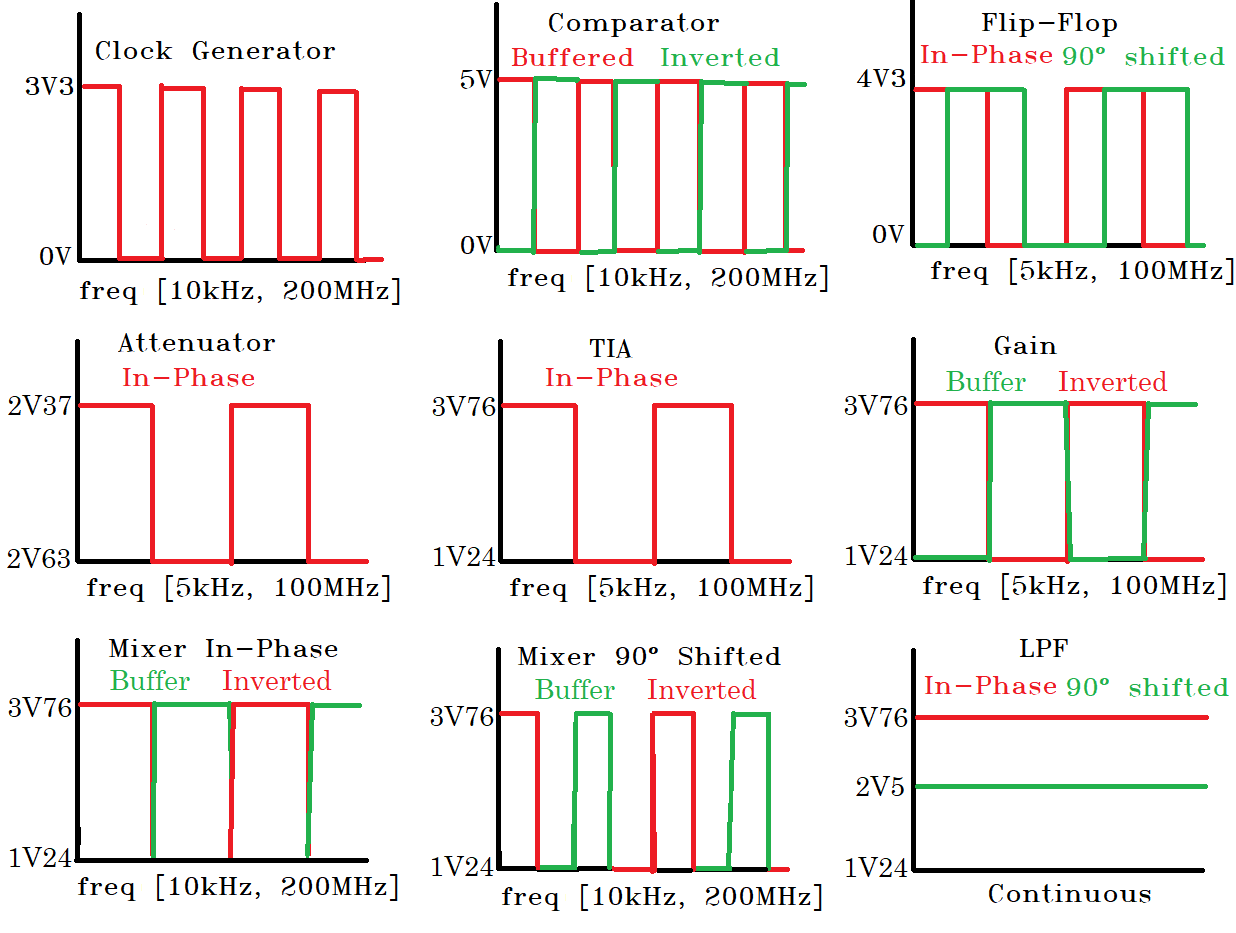
\includegraphics[width=1\textwidth]{IFCPracticalExample}
    \caption{Signal behavior for every electronical modules of the impedance-sensing device when measuring a 1k$\Omega$ resistor with a 10k$\Omega$ feedback resistor at the PGA.}
    \label{fig:IFCPracticalExample}
\end{figure}
By calculating the difference of these signals from the middle of the power-supplies, it is possible to obtain the real and imaginary components. the real component is 1.265 while the imaginary component is 0. Since the SUT in this case is a resistor, which has only a real component for the impedance, the conversion from the square spectroscopy to a sine spectroscopy doesn't modify the results, as described in the proof below. 
\begin{proof}
Since this is a 1k$\Omega$ resistor, the real component should be 1000 and the imaginary component should be 0. 
    \begin{align*}
        \Re(V_{PSD-\omega_0}) & = \frac{1}{2}\frac{6}{\pi^2} \frac{V_0 R_f}{A} \displaystyle\sum_{n=1,3,5,7...} ^{\infty} \frac{\cos(\theta(n \omega_0))}{n^2\lvert Z \rvert (n \omega_0)}\nonumber\\
        1.265 & = \frac{1}{2} \frac{6}{\pi^2} \frac{4.3 * 4 700}{17} \displaystyle\sum_{n=1,3,5,7...} ^{\infty} \frac{\cos(0 ^\circ)}{n^2 1000}\nonumber\\
        1.265 & = \frac{1}{2} \frac{6}{\pi^2} 2529 \displaystyle\sum_{n=1,3,5,7...} ^{\infty} \frac{1}{n^2 1000}\nonumber\\
        1.265 & = \frac{1}{2} \frac{2529}{1000}\nonumber\\ 
        1000 & = 1000\nonumber &&\qedhere
    \end{align*}
\end{proof}
\autoref{eq:CorrectedMagnitude} and \autoref{eq:CorrectedPhase} can thus be used directly with \autoref{eq:RealPSD} and \autoref{eq:ImPSD} to calculate the magnitude and phase of the SUT's impedance. A magnitude of 1000$\Omega$ and a phase of 0$^\circ$ are calculated, which is exactly what was sought for the 1k$\Omega$ resistor.  \par

\subsection{General example}
Another more general example can be illustrated for a complex system involving a series capacitor and resistor of values 1nF and 1k$\Omega$ excited by an input square signal of frequency 100kHz with a transimpedance of the PGA of 10k$\Omega$. The impedance magnitude and phase of the SUT would then be 1880$\Omega$ and -57.86 $^\circ$. Here is the proof below:

\begin{proof}
    Knowing that the impedance magnitude and phase for the fundamental and three first harmonics are: ($n=1$) 1880$\Omega$ and -57.86 $^\circ$, ($n=3$) 1132$\Omega$ and -27.95 $^\circ$, ($n=5$) 1049$\Omega$ and -17.66 $^\circ$, ($n=7$) 1025$\Omega$ and -12.81 $^\circ$. The real and imaginary components sampled by the ADCs would be:
    \begin{align*}
       \Re(V_{PSD-\omega_0}) &= \frac{1}{2} \frac{6}{\pi^2} \frac{V_0 R_f}{A} \displaystyle\sum_{n=1,3,5,7...} ^{\infty} \frac{\cos(\theta(n \omega_0))}{n^2\lvert Z \rvert (n \omega_0)}\nonumber\\
        &= \frac{1}{2} \frac{6}{\pi^2} 2529 [\frac{\cos(57.86 ^\circ)}{1880} + \frac{\cos(27.95^\circ)}{3^2 * 1132} + \frac{\cos(17.66 ^\circ)}{5^2 * 1049} + \frac{\cos(12.81 ^\circ)}{7^2 * 1025} + \dots]\nonumber\\
        &= -0.2350 \nonumber
       \end{align*}
     \begin{align*}
       \Im(V_{PSD-\omega_0}) &= \frac{1}{2} \frac{6}{\pi^2} \frac{V_0 R_f}{A} \displaystyle\sum_{n=1,3,5,7...} ^{\infty} \frac{\sin(\theta(n \omega_0))}{n^2\lvert Z \rvert (n \omega_0)}\nonumber\\
        &= \frac{1}{2} \frac{6}{\pi^2} 2529 [\frac{\sin(57.86 ^\circ)}{1880} + \frac{\sin(27.95^\circ)}{3^2 * 1132} + \frac{\sin(17.66 ^\circ)}{5^2 * 1049} + \frac{\sin(12.81 ^\circ)}{7^2 * 1025} + \dots]\nonumber\\
        &= 0.1991\nonumber
    \end{align*}
    Now these real and imaginary square components must be corrected using the rules described in \citep{Subhan2019} following \autoref{eq:correctionReal}. The coefficients $\Re(V_{PSD-\omega_0})$ and $\Im(V_{PSD-\omega_0})$ at the harmonics frequency must have been sampled beforehand. $\Re(V_{PSD-3\omega_0}=-0.4865$, $\Re(V_{PSD-5\omega_0}=-0.5489$, $\Re(V_{PSD-7\omega_0}=-0.5698$, $\Im(V_{PSD-3\omega_0}=0.1906$, $\Im(V_{PSD-5\omega_0}=0.1332$, $\Im(V_{PSD-7\omega_0}=0.0994$. 
    \begin{align*}
       \Re(V_{sine-\omega_0}) &= \frac{1}{2} \frac{6}{\pi^2} \frac{V_0}{A} R_f [ \displaystyle\sum_{n=1,3,5,7...} ^{\infty} \frac{\cos(\theta(n \omega_0))}{n^2\lvert Z \rvert (n \omega_0)} - \displaystyle\sum_{n=3,5,7...} ^{\infty} \frac{\cos(\theta(n \omega_0))}{n^2\lvert Z \rvert (n \omega_0)}]\nonumber\\
       &= \Re(V_{PSD-\omega_0}) - \frac{1}{3^2}\Re(V_{PSD-3\omega_0}) - \frac{1}{5^2}\Re(V_{PSD-5\omega_0}) - \frac{1}{7^2}\Re(V_{PSD-7\omega_0}) + \dots\nonumber\\
       &=  -0.2350 + \frac{0.4865}{9} + \frac{0.5489}{25} + \frac{0.5698}{49} + \dots\nonumber\\
       &= -0.1474\nonumber
   \end{align*}
   \begin{align*}
       \Im(V_{sine-\omega_0}) &= \frac{1}{2} \frac{6}{\pi^2} \frac{V_0}{A} R_f [ \displaystyle\sum_{n=1,3,5,7...} ^{\infty} \frac{\sin(\theta(n \omega_0))}{n^2\lvert Z \rvert (n \omega_0)} - \displaystyle\sum_{n=3,5,7...} ^{\infty} \frac{\sin(\theta(n \omega_0))}{n^2\lvert Z \rvert (n \omega_0)}]\nonumber\\
       &= \Im(V_{PSD-\omega_0}) + \frac{1}{3^2}\Im(V_{PSD-3\omega_0}) - \frac{1}{5^2}\Im(V_{PSD-5\omega_0}) + \frac{1}{7^2}\Im(V_{PSD-7\omega_0}) + \dots\nonumber\\
       &=  0.1991 + \frac{0.1906}{9} - \frac{0.1332}{25} + \frac{0.0994}{49} + \dots\nonumber\\
       &= 0.2170\nonumber &&\qedhere
    \end{align*}
\end{proof}
The impedance magnitude is thus deduced the same way as the previous proof to be 1 837 $\Omega$, only 2.3\% away from the theoretical value of 1880 $\Omega$. The impedance phase is -55.8 $^{\circ}$, only 3.6\% away from the theoretical value of -57.86 $^\circ$. These errors are quite low considering that only the first 3 harmonics were subtracted from the square spectroscopy. When more harmonics are considered, the error can go as low as 1\% for the magnitude and 1.5\% for the phase.